% Options for packages loaded elsewhere
\PassOptionsToPackage{unicode}{hyperref}
\PassOptionsToPackage{hyphens}{url}
%
\documentclass[
  12pt,
]{article}
\usepackage{amsmath,amssymb}
\usepackage{lmodern}
\usepackage{iftex}
\ifPDFTeX
  \usepackage[T1]{fontenc}
  \usepackage[utf8]{inputenc}
  \usepackage{textcomp} % provide euro and other symbols
\else % if luatex or xetex
  \usepackage{unicode-math}
  \defaultfontfeatures{Scale=MatchLowercase}
  \defaultfontfeatures[\rmfamily]{Ligatures=TeX,Scale=1}
  \setmainfont[]{Arial}
\fi
% Use upquote if available, for straight quotes in verbatim environments
\IfFileExists{upquote.sty}{\usepackage{upquote}}{}
\IfFileExists{microtype.sty}{% use microtype if available
  \usepackage[]{microtype}
  \UseMicrotypeSet[protrusion]{basicmath} % disable protrusion for tt fonts
}{}
\makeatletter
\@ifundefined{KOMAClassName}{% if non-KOMA class
  \IfFileExists{parskip.sty}{%
    \usepackage{parskip}
  }{% else
    \setlength{\parindent}{0pt}
    \setlength{\parskip}{6pt plus 2pt minus 1pt}}
}{% if KOMA class
  \KOMAoptions{parskip=half}}
\makeatother
\usepackage{xcolor}
\usepackage[margin=0.5in]{geometry}
\usepackage{color}
\usepackage{fancyvrb}
\newcommand{\VerbBar}{|}
\newcommand{\VERB}{\Verb[commandchars=\\\{\}]}
\DefineVerbatimEnvironment{Highlighting}{Verbatim}{commandchars=\\\{\}}
% Add ',fontsize=\small' for more characters per line
\usepackage{framed}
\definecolor{shadecolor}{RGB}{248,248,248}
\newenvironment{Shaded}{\begin{snugshade}}{\end{snugshade}}
\newcommand{\AlertTok}[1]{\textcolor[rgb]{0.94,0.16,0.16}{#1}}
\newcommand{\AnnotationTok}[1]{\textcolor[rgb]{0.56,0.35,0.01}{\textbf{\textit{#1}}}}
\newcommand{\AttributeTok}[1]{\textcolor[rgb]{0.77,0.63,0.00}{#1}}
\newcommand{\BaseNTok}[1]{\textcolor[rgb]{0.00,0.00,0.81}{#1}}
\newcommand{\BuiltInTok}[1]{#1}
\newcommand{\CharTok}[1]{\textcolor[rgb]{0.31,0.60,0.02}{#1}}
\newcommand{\CommentTok}[1]{\textcolor[rgb]{0.56,0.35,0.01}{\textit{#1}}}
\newcommand{\CommentVarTok}[1]{\textcolor[rgb]{0.56,0.35,0.01}{\textbf{\textit{#1}}}}
\newcommand{\ConstantTok}[1]{\textcolor[rgb]{0.00,0.00,0.00}{#1}}
\newcommand{\ControlFlowTok}[1]{\textcolor[rgb]{0.13,0.29,0.53}{\textbf{#1}}}
\newcommand{\DataTypeTok}[1]{\textcolor[rgb]{0.13,0.29,0.53}{#1}}
\newcommand{\DecValTok}[1]{\textcolor[rgb]{0.00,0.00,0.81}{#1}}
\newcommand{\DocumentationTok}[1]{\textcolor[rgb]{0.56,0.35,0.01}{\textbf{\textit{#1}}}}
\newcommand{\ErrorTok}[1]{\textcolor[rgb]{0.64,0.00,0.00}{\textbf{#1}}}
\newcommand{\ExtensionTok}[1]{#1}
\newcommand{\FloatTok}[1]{\textcolor[rgb]{0.00,0.00,0.81}{#1}}
\newcommand{\FunctionTok}[1]{\textcolor[rgb]{0.00,0.00,0.00}{#1}}
\newcommand{\ImportTok}[1]{#1}
\newcommand{\InformationTok}[1]{\textcolor[rgb]{0.56,0.35,0.01}{\textbf{\textit{#1}}}}
\newcommand{\KeywordTok}[1]{\textcolor[rgb]{0.13,0.29,0.53}{\textbf{#1}}}
\newcommand{\NormalTok}[1]{#1}
\newcommand{\OperatorTok}[1]{\textcolor[rgb]{0.81,0.36,0.00}{\textbf{#1}}}
\newcommand{\OtherTok}[1]{\textcolor[rgb]{0.56,0.35,0.01}{#1}}
\newcommand{\PreprocessorTok}[1]{\textcolor[rgb]{0.56,0.35,0.01}{\textit{#1}}}
\newcommand{\RegionMarkerTok}[1]{#1}
\newcommand{\SpecialCharTok}[1]{\textcolor[rgb]{0.00,0.00,0.00}{#1}}
\newcommand{\SpecialStringTok}[1]{\textcolor[rgb]{0.31,0.60,0.02}{#1}}
\newcommand{\StringTok}[1]{\textcolor[rgb]{0.31,0.60,0.02}{#1}}
\newcommand{\VariableTok}[1]{\textcolor[rgb]{0.00,0.00,0.00}{#1}}
\newcommand{\VerbatimStringTok}[1]{\textcolor[rgb]{0.31,0.60,0.02}{#1}}
\newcommand{\WarningTok}[1]{\textcolor[rgb]{0.56,0.35,0.01}{\textbf{\textit{#1}}}}
\usepackage{longtable,booktabs,array}
\usepackage{calc} % for calculating minipage widths
% Correct order of tables after \paragraph or \subparagraph
\usepackage{etoolbox}
\makeatletter
\patchcmd\longtable{\par}{\if@noskipsec\mbox{}\fi\par}{}{}
\makeatother
% Allow footnotes in longtable head/foot
\IfFileExists{footnotehyper.sty}{\usepackage{footnotehyper}}{\usepackage{footnote}}
\makesavenoteenv{longtable}
\usepackage{graphicx}
\makeatletter
\def\maxwidth{\ifdim\Gin@nat@width>\linewidth\linewidth\else\Gin@nat@width\fi}
\def\maxheight{\ifdim\Gin@nat@height>\textheight\textheight\else\Gin@nat@height\fi}
\makeatother
% Scale images if necessary, so that they will not overflow the page
% margins by default, and it is still possible to overwrite the defaults
% using explicit options in \includegraphics[width, height, ...]{}
\setkeys{Gin}{width=\maxwidth,height=\maxheight,keepaspectratio}
% Set default figure placement to htbp
\makeatletter
\def\fps@figure{htbp}
\makeatother
\setlength{\emergencystretch}{3em} % prevent overfull lines
\providecommand{\tightlist}{%
  \setlength{\itemsep}{0pt}\setlength{\parskip}{0pt}}
\setcounter{secnumdepth}{-\maxdimen} % remove section numbering
\ifLuaTeX
  \usepackage{selnolig}  % disable illegal ligatures
\fi
\IfFileExists{bookmark.sty}{\usepackage{bookmark}}{\usepackage{hyperref}}
\IfFileExists{xurl.sty}{\usepackage{xurl}}{} % add URL line breaks if available
\urlstyle{same} % disable monospaced font for URLs
\hypersetup{
  pdftitle={R Markdown Tutorial Demo},
  pdfauthor={John Doe},
  hidelinks,
  pdfcreator={LaTeX via pandoc}}

\title{R Markdown Tutorial Demo}
\author{John Doe}
\date{21/11/2016}

\begin{document}
\maketitle

\hypertarget{preamble}{%
\subsection{Preamble}\label{preamble}}

\hypertarget{packages}{%
\subsubsection{Packages}\label{packages}}

\begin{Shaded}
\begin{Highlighting}[]
\FunctionTok{library}\NormalTok{(dplyr) }\CommentTok{\# for data manipulation}
\FunctionTok{library}\NormalTok{(pander) }\CommentTok{\# to create pretty tables}
\end{Highlighting}
\end{Shaded}

\hypertarget{data-exploration}{%
\subsection{Data Exploration}\label{data-exploration}}

A preliminary investigation into the biodiversity of Edinburgh, using
data from the NBN Gateway \url{https://data.nbn.org.uk/}.

\hypertarget{what-is-the-species-richness-across-taxonomic-groups}{%
\subsubsection{What is the species richness across taxonomic
groups?}\label{what-is-the-species-richness-across-taxonomic-groups}}

A table of species richness:

\begin{Shaded}
\begin{Highlighting}[]
\NormalTok{richness }\OtherTok{\textless{}{-}} 
\NormalTok{  edidiv }\SpecialCharTok{\%\textgreater{}\%}
  \FunctionTok{group\_by}\NormalTok{(taxonGroup) }\SpecialCharTok{\%\textgreater{}\%}
  \FunctionTok{summarise}\NormalTok{(}\AttributeTok{Species\_richness =} \FunctionTok{n\_distinct}\NormalTok{(taxonName)) }

\FunctionTok{pander}\NormalTok{(richness)}
\end{Highlighting}
\end{Shaded}

\begin{longtable}[]{@{}
  >{\centering\arraybackslash}p{(\columnwidth - 2\tabcolsep) * \real{0.2639}}
  >{\centering\arraybackslash}p{(\columnwidth - 2\tabcolsep) * \real{0.2639}}@{}}
\toprule()
\begin{minipage}[b]{\linewidth}\centering
taxonGroup
\end{minipage} & \begin{minipage}[b]{\linewidth}\centering
Species\_richness
\end{minipage} \\
\midrule()
\endhead
Beetle & 37 \\
Bird & 86 \\
Butterfly & 25 \\
Dragonfly & 11 \\
Flowering.Plants & 521 \\
Fungus & 219 \\
Hymenopteran & 112 \\
Lichen & 94 \\
Liverwort & 40 \\
Mammal & 33 \\
Mollusc & 97 \\
\bottomrule()
\end{longtable}

A barplot of the table above:

\begin{Shaded}
\begin{Highlighting}[]
\FunctionTok{barplot}\NormalTok{(richness}\SpecialCharTok{$}\NormalTok{Species\_richness, }
        \AttributeTok{names.arg =}\NormalTok{ richness}\SpecialCharTok{$}\NormalTok{taxonGroup, }
        \AttributeTok{xlab=}\StringTok{"Taxa"}\NormalTok{, }\AttributeTok{ylab=}\StringTok{"Number of species"}\NormalTok{, }
        \AttributeTok{ylim=}\FunctionTok{c}\NormalTok{(}\DecValTok{0}\NormalTok{,}\DecValTok{600}\NormalTok{)}
\NormalTok{        ) }
\end{Highlighting}
\end{Shaded}

\begin{center}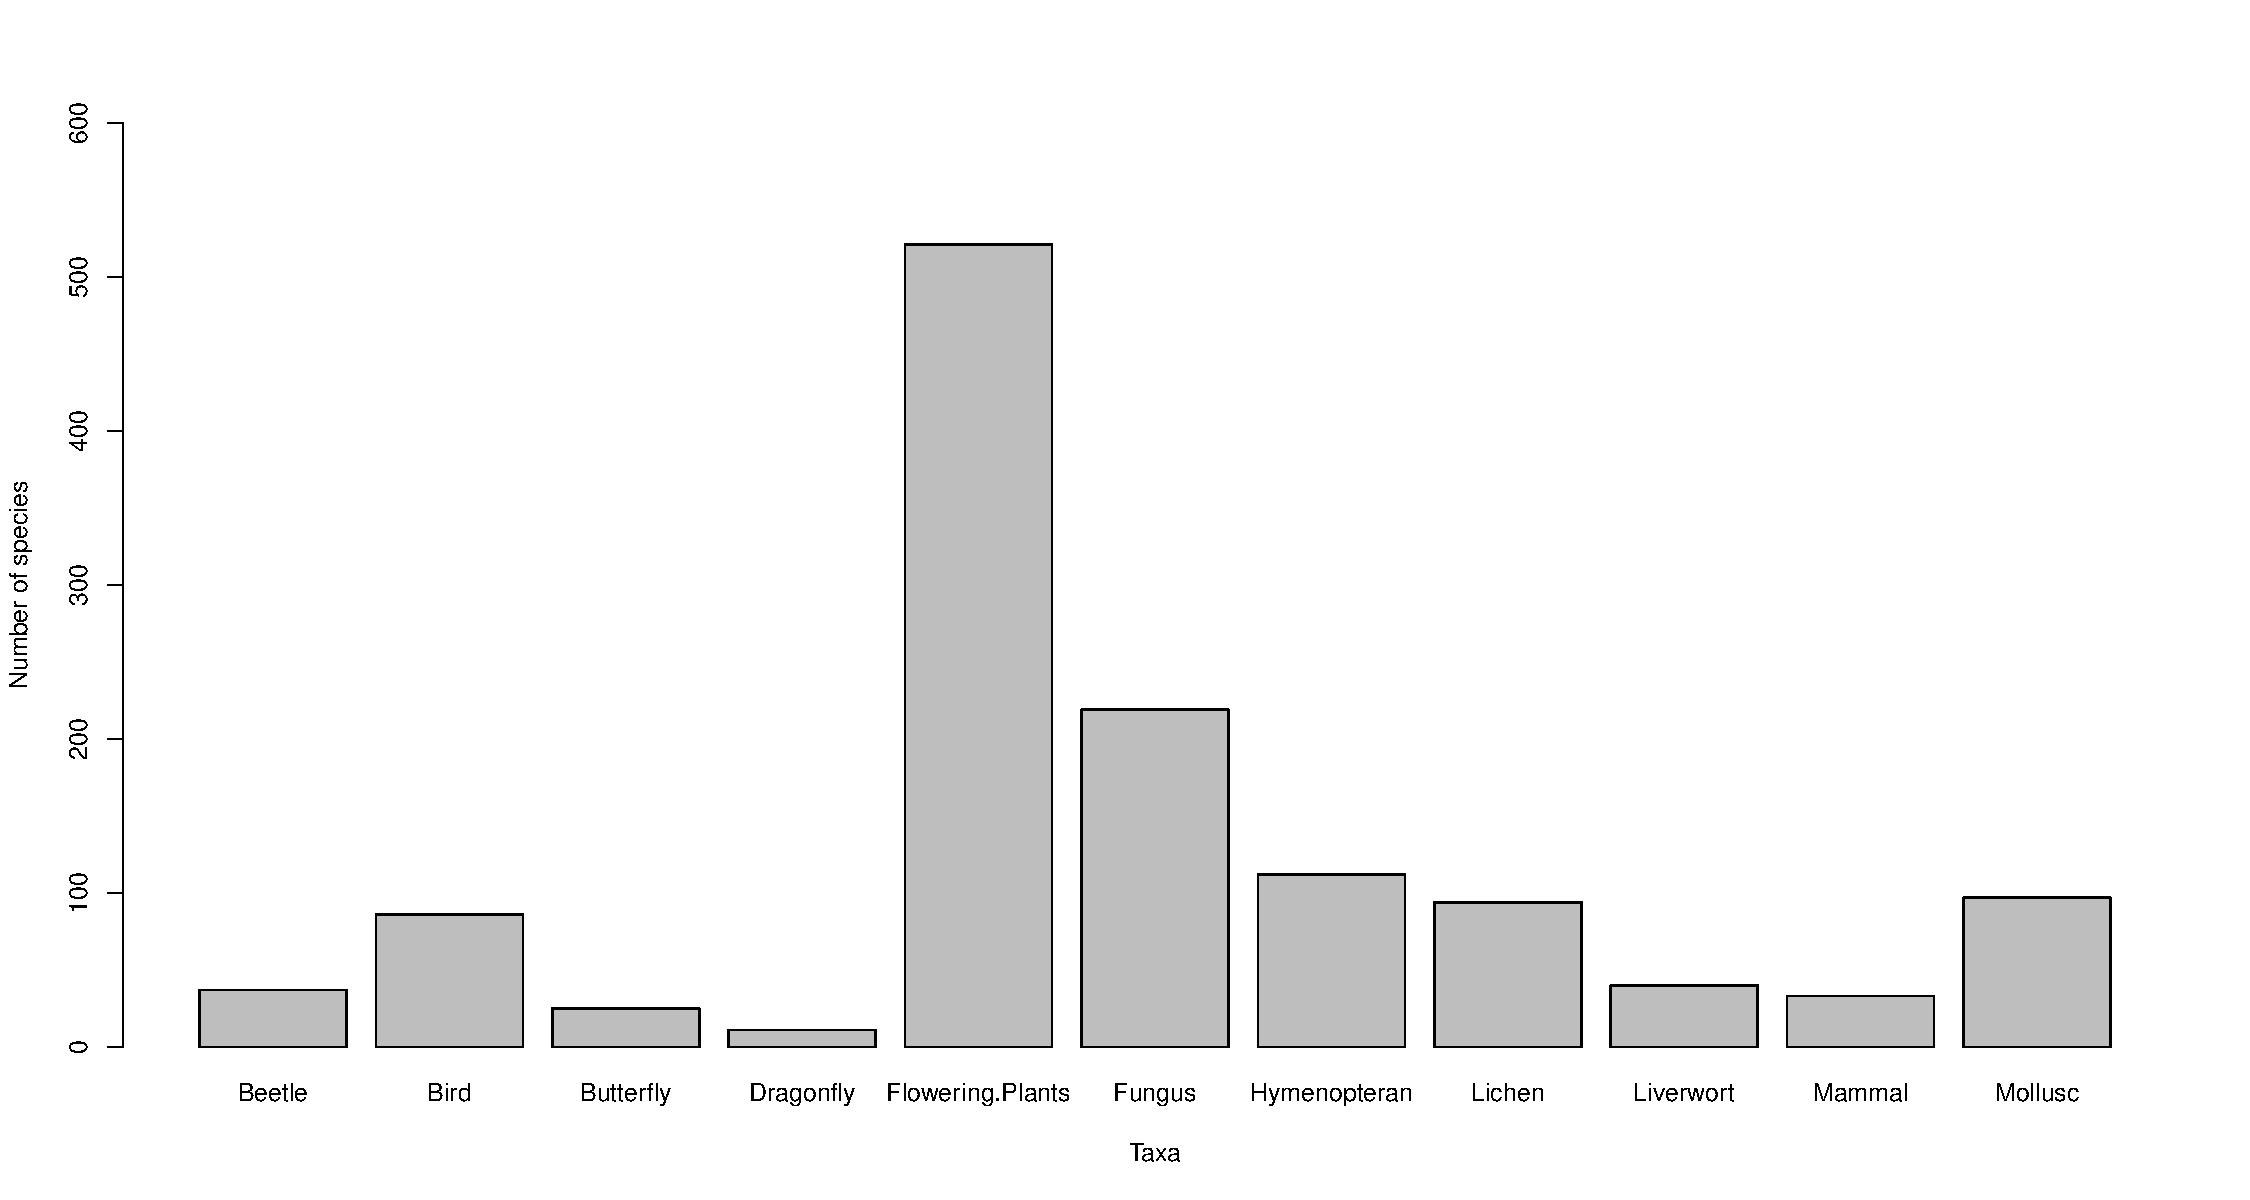
\includegraphics{RMarkdown_Tutorial_Demo_Rmd_files/figure-latex/unnamed-chunk-4-1} \end{center}

\hypertarget{what-is-the-most-common-species-in-each-taxonomic-group}{%
\subsubsection{What is the most common species in each taxonomic
group?}\label{what-is-the-most-common-species-in-each-taxonomic-group}}

A table of the most common species:

\begin{Shaded}
\begin{Highlighting}[]
\CommentTok{\#Create a vector of most abundant species per taxa}
\NormalTok{max\_abund }\OtherTok{\textless{}{-}}
\NormalTok{  edidiv }\SpecialCharTok{\%\textgreater{}\%}
    \FunctionTok{group\_by}\NormalTok{(taxonGroup) }\SpecialCharTok{\%\textgreater{}\%}
    \FunctionTok{summarise}\NormalTok{(}\AttributeTok{taxonName =} \FunctionTok{names}\NormalTok{(}\FunctionTok{which.max}\NormalTok{(}\FunctionTok{table}\NormalTok{(taxonName))))}

\CommentTok{\#Add the vector to the data frame}
\NormalTok{richness\_abund }\OtherTok{\textless{}{-}}
\FunctionTok{inner\_join}\NormalTok{(richness, max\_abund, }\AttributeTok{by =} \StringTok{"taxonGroup"}\NormalTok{)}
\NormalTok{richness\_abund }\OtherTok{\textless{}{-}} \FunctionTok{rename}\NormalTok{(richness\_abund, }\AttributeTok{Most\_abundant =}\NormalTok{  taxonName, }\AttributeTok{Taxon =}\NormalTok{ taxonGroup)}
\end{Highlighting}
\end{Shaded}

\begin{Shaded}
\begin{Highlighting}[]
\NormalTok{richness\_abund }\OtherTok{\textless{}{-}} \FunctionTok{rename}\NormalTok{(richness\_abund, }
                        \StringTok{"Most Abundant"} \OtherTok{=}\NormalTok{ Most\_abundant,}
                        \StringTok{"Species Richness"} \OtherTok{=}\NormalTok{ Species\_richness) }\CommentTok{\#Change the column names}
\FunctionTok{emphasize.italics.cols}\NormalTok{(}\DecValTok{3}\NormalTok{) }\CommentTok{\#Make the 3rd column italics}
\FunctionTok{pander}\NormalTok{(richness\_abund) }\CommentTok{\#Create a table}
\end{Highlighting}
\end{Shaded}

\begin{longtable}[]{@{}
  >{\centering\arraybackslash}p{(\columnwidth - 4\tabcolsep) * \real{0.2639}}
  >{\centering\arraybackslash}p{(\columnwidth - 4\tabcolsep) * \real{0.2639}}
  >{\centering\arraybackslash}p{(\columnwidth - 4\tabcolsep) * \real{0.4306}}@{}}
\toprule()
\begin{minipage}[b]{\linewidth}\centering
Taxon
\end{minipage} & \begin{minipage}[b]{\linewidth}\centering
Species Richness
\end{minipage} & \begin{minipage}[b]{\linewidth}\centering
Most Abundant
\end{minipage} \\
\midrule()
\endhead
Beetle & 37 & \emph{Coccinella septempunctata} \\
Bird & 86 & \emph{Turdus merula} \\
Butterfly & 25 & \emph{Maniola jurtina} \\
Dragonfly & 11 & \emph{Ischnura elegans} \\
Flowering.Plants & 521 & \emph{Urtica dioica} \\
Fungus & 219 & \emph{Auricularia auricula-judae} \\
Hymenopteran & 112 & \emph{Bombus (Bombus) terrestris} \\
Lichen & 94 & \emph{Xanthoria parietina} \\
Liverwort & 40 & \emph{Lophocolea bidentata} \\
Mammal & 33 & \emph{Sciurus carolinensis} \\
Mollusc & 97 & \emph{Cornu aspersum} \\
\bottomrule()
\end{longtable}

kable(max\_abund)

\end{document}
